\documentclass[11pt,compress,t,notes=noshow, xcolor=table]{beamer}
\usepackage[]{graphicx}\usepackage[]{color}
% maxwidth is the original width if it is less than linewidth
% otherwise use linewidth (to make sure the graphics do not exceed the margin)
\makeatletter
\def\maxwidth{ %
  \ifdim\Gin@nat@width>\linewidth
    \linewidth
  \else
    \Gin@nat@width
  \fi
}
\makeatother

\newcommand{\citebutton}[2]{%
\beamergotobutton{\href{#2}{#1}}%
}

\newcommand{\blu}[1]{\textcolor{blue}{#1}}
\newcommand{\org}[1]{\textcolor{orange}{#1}}
\newcommand{\ques}{\textbf{\textcolor{red}{Question:  }}}
\newcommand{\questionssofar}{\begin{frame}\frametitle{Any questions?}\end{frame}}

\newcommand\warning{%
 \makebox[1.4em][c]{%
 \makebox[0pt][c]{\raisebox{.1em}{\scriptsize!}}%
 \makebox[0pt][c]{\color{red}\normalsize$\bigtriangleup$}}}%

\definecolor{fgcolor}{rgb}{0.345, 0.345, 0.345}
\newcommand{\hlnum}[1]{\textcolor[rgb]{0.686,0.059,0.569}{#1}}%
\newcommand{\hlstr}[1]{\textcolor[rgb]{0.192,0.494,0.8}{#1}}%
\newcommand{\hlcom}[1]{\textcolor[rgb]{0.678,0.584,0.686}{\textit{#1}}}%
\newcommand{\hlopt}[1]{\textcolor[rgb]{0,0,0}{#1}}%
\newcommand{\hlstd}[1]{\textcolor[rgb]{0.345,0.345,0.345}{#1}}%
\newcommand{\hlkwa}[1]{\textcolor[rgb]{0.161,0.373,0.58}{\textbf{#1}}}%
\newcommand{\hlkwb}[1]{\textcolor[rgb]{0.69,0.353,0.396}{#1}}%
\newcommand{\hlkwc}[1]{\textcolor[rgb]{0.333,0.667,0.333}{#1}}%
\newcommand{\hlkwd}[1]{\textcolor[rgb]{0.737,0.353,0.396}{\textbf{#1}}}%
\let\hlipl\hlkwb

\usepackage{framed}
\makeatletter
\newenvironment{kframe}{%
 \def\at@end@of@kframe{}%
 \ifinner\ifhmode%
  \def\at@end@of@kframe{\end{minipage}}%
  \begin{minipage}{\columnwidth}%
 \fi\fi%
 \def\FrameCommand##1{\hskip\@totalleftmargin \hskip-\fboxsep
 \colorbox{shadecolor}{##1}\hskip-\fboxsep
     % There is no \\@totalrightmargin, so:
     \hskip-\linewidth \hskip-\@totalleftmargin \hskip\columnwidth}%
 \MakeFramed {\advance\hsize-\width
   \@totalleftmargin\z@ \linewidth\hsize
   \@setminipage}}%
 {\par\unskip\endMakeFramed%
 \at@end@of@kframe}
\makeatother

\definecolor{shadecolor}{rgb}{.97, .97, .97}
\definecolor{messagecolor}{rgb}{0, 0, 0}
\definecolor{warningcolor}{rgb}{1, 0, 1}
\definecolor{errorcolor}{rgb}{1, 0, 0}
\newenvironment{knitrout}{}{} % an empty environment to be redefined in TeX

\usepackage{alltt}
\newcommand{\SweaveOpts}[1]{}  % do not interfere with LaTeX
\newcommand{\SweaveInput}[1]{} % because they are not real TeX commands
\newcommand{\Sexpr}[1]{}       % will only be parsed by R
\newcommand{\xmark}{\ding{55}}%


\usepackage[english]{babel}
\usepackage[utf8]{inputenc}

\usepackage{dsfont}
\usepackage{verbatim}
\usepackage{amsmath}
\usepackage{amsfonts}
\usepackage{amssymb}
\usepackage{bm}
\usepackage{csquotes}
\usepackage{multirow}
\usepackage{longtable}
\usepackage{booktabs}
\usepackage{enumerate}
\usepackage[absolute,overlay]{textpos}
\usepackage{psfrag}
\usepackage{algorithm}
\usepackage{algpseudocode}
\usepackage{eqnarray}
\usepackage{arydshln}
\usepackage{tabularx}
\usepackage{placeins}
\usepackage{tikz}
\usepackage{setspace}
\usepackage{colortbl}
\usepackage{mathtools}
\usepackage{wrapfig}
\usepackage{bm}
\usepackage{amsmath}
\usepackage{pifont}

\usetikzlibrary{shapes.multipart,shapes,arrows,automata,positioning,calc,chains,trees, shadows}
\tikzset{
  %Define standard arrow tip
  >=stealth',
  %Define style for boxes
  punkt/.style={
    rectangle,
    rounded corners,
    draw=black, very thick,
    text width=6.5em,
    minimum height=2em,
    text centered},
  % Define arrow style
  pil/.style={
    ->,
    thick,
    shorten <=2pt,
    shorten >=2pt,}
}

\tikzstyle{vec}=[draw, rectangle, fill = white, minimum width=5mm, minimum height=1cm, inner sep = 2pt]

\usepackage{subfig}

% Defines macros and environments
\usepackage{../../style/lmu-lecture}


\let\code=\texttt
\let\proglang=\textsf

\setkeys{Gin}{width=0.9\textwidth}

\setbeamertemplate{frametitle}{\expandafter\uppercase\expandafter\insertframetitle}

\usepackage{bbm}
% basic latex stuff
\newcommand{\pkg}[1]{{\fontseries{b}\selectfont #1}} %fontstyle for R packages
\newcommand{\lz}{\vspace{0.5cm}} %vertical space
\newcommand{\dlz}{\vspace{1cm}} %double vertical space
\newcommand{\oneliner}[1] % Oneliner for important statements
{\begin{block}{}\begin{center}\begin{Large}#1\end{Large}\end{center}\end{block}}


%new environments
\newenvironment{vbframe}  %frame with breaks and verbatim
{
 \begin{frame}[containsverbatim,allowframebreaks]
}
{
\end{frame}
}

\newenvironment{vframe}  %frame with verbatim without breaks (to avoid numbering one slided frames)
{
 \begin{frame}[containsverbatim]
}
{
\end{frame}
}

\newenvironment{blocki}[1]   % itemize block
{
 \begin{block}{#1}\begin{itemize}
}
{
\end{itemize}\end{block}
}

\newenvironment{fragileframe}[2]{  %fragile frame with framebreaks
\begin{frame}[allowframebreaks, fragile, environment = fragileframe]
\frametitle{#1}
#2}
{\end{frame}}


\newcommand{\myframe}[2]{  %short for frame with framebreaks
\begin{frame}[allowframebreaks]
\frametitle{#1}
#2
\end{frame}}

\newcommand{\remark}[1]{
  \textbf{Remark:} #1
}


\newenvironment{deleteframe}
{
\begingroup
\usebackgroundtemplate{
\includegraphics[width=\paperwidth,height=\paperheight]{../style/color/red.png}}
 \begin{frame}
}
{
\end{frame}
\endgroup
}
\newenvironment{simplifyframe}
{
\begingroup
\usebackgroundtemplate{
\includegraphics[width=\paperwidth,height=\paperheight]{../style/color/yellow.png}}
 \begin{frame}
}
{
\end{frame}
\endgroup
}\newenvironment{draftframe}
{
\begingroup
\usebackgroundtemplate{
\includegraphics[width=\paperwidth,height=\paperheight]{../style/color/green.jpg}}
 \begin{frame}
}
{
\end{frame}
\endgroup
}
% https://tex.stackexchange.com/a/261480: textcolor that works in mathmode
\makeatletter
\renewcommand*{\@textcolor}[3]{%
  \protect\leavevmode
  \begingroup
    \color#1{#2}#3%
  \endgroup
}
\makeatother





\input{../../latex-math/basic-math.tex}
\input{../../latex-math/basic-ml.tex}

\newcommand{\titlefigure}{figure/bert.jpeg}
\newcommand{\learninggoals}{
\item Understand how impactful this architecture was
\item See how this changed research in the field}

\title{Using the Transformer}
% \author{}
\institute{\href{https://slds-lmu.github.io/lecture_dl4nlp/}{slds-lmu.github.io/lecture\_dl4nlp}}
\date{}

\begin{document}
\lecturechapter{BERT -- Implications for future work}
\lecture{Deep Learning for NLP}

% ------------------------------------------------------------------------------

\begin{frame}{English Centricity of NLP}

\vfill

	\begin{itemize}
		\item BERT trained on a corpus of English text
		\item More importantly: Also only evaluated on English benchmarks (obviously)\\	
					\href{https://gluebenchmark.com/}{\beamergotobutton{GLUE}}
					\href{https://rajpurkar.github.io/SQuAD-explorer/}{\beamergotobutton{SQUAD}}
					\href{https://www.qizhexie.com/data/RACE_leaderboard.html}{\beamergotobutton{RACE}}
		\item Devlin et al. (2019) published different (monolingual) models, but only varying in size, not in language
		\item Later: Multilingual BERT model \href{https://github.com/google-research/bert/blob/master/multilingual.md}{\beamergotobutton{mBERT}} for 100+ languages
		\item This leads to a shared embedding space for all the languages included in the model
		\item Before this: Need for alignment of separately learned embedding spaces
	\end{itemize}

\vfill

\end{frame}

% ------------------------------------------------------------------------------

\begin{frame}{BERTs for all languages}

\vfill

\begin{itemize}
	\item The breakthrough performance of BERT in the English Language triggered a wave of new
				BERT models in different languages. Just to name a few:
			\begin{itemize}
				\item \href{https://huggingface.co/bert-base-german-cased}{\beamergotobutton{German BERT}}
				\item \href{https://huggingface.co/flaubert/flaubert_base_cased}{\beamergotobutton{FlauBERT (French)}}
				\item \href{https://huggingface.co/dccuchile/bert-base-spanish-wwm-cased}{\beamergotobutton{BETO (Spanish)}}
				\item \href{https://huggingface.co/GroNLP/bert-base-dutch-cased}{\beamergotobutton{BERTje (Dutch)}}
				\item \href{https://huggingface.co/bert-base-chinese}{\beamergotobutton{Chinese BERT}}
				\item \href{https://huggingface.co/DeepPavlov/rubert-base-cased}{\beamergotobutton{RuBERT (Russian)}}
				\item \href{https://huggingface.co/dbmdz/bert-base-italian-cased}{\beamergotobutton{Italian BERT}}
				\item ...
			\end{itemize}
\end{itemize}
	
\vfill

\end{frame}

% ------------------------------------------------------------------------------

\begin{frame}{Pretrain-finetune + Transformer backbone}

\vfill

	\begin{itemize}
		\item Before BERT: 
			\begin{itemize}
				\item ELMo (and other specialized architectures) very popular
				\item Examples (also CNNs): 
							\href{https://arxiv.org/abs/1408.5882}{\beamergotobutton{Kim, 2014}} 
							\href{https://proceedings.neurips.cc/paper/2015/file/250cf8b51c773f3f8dc8b4be867a9a02-Paper.pdf}{\beamergotobutton{Zhang et al., 2016}}
			\end{itemize}
		\item After BERT:
			\begin{itemize}
				\item Using a pre-trained model and fine-tuning it is the de-facto standard
				\item CNNs and RNNs rarely used, different variants of the transformer or other self-attention based mechanisms are the backbone of nearly every architecture
			\end{itemize}
	\end{itemize}

\vfill

\end{frame}

% ------------------------------------------------------------------------------

\begin{frame}{BERTology \href{https://aclanthology.org/2020.tacl-1.54.pdf}{\beamergotobutton{Rodgers et al., 2020}}}

\vfill

\textbf{Post-BERT architectures:}

\begin{itemize}
\item Most architectures still rely on either an encoder- \textit{or} a decoder-style type of model (e.g. \href{https://cdn.openai.com/better-language-models/language_models_are_unsupervised_multitask_learners.pdf}{\beamergotobutton{GPT2}}, \href{https://arxiv.org/pdf/1906.08237.pdf}{\beamergotobutton{XLNet}})
\item \textit{BERTology:} Many papers/models which aim at ..
			\begin{itemize}
				\item .. explanining BERT (e.g. \href{https://arxiv.org/pdf/1906.02715.pdf}{\beamergotobutton{Coenen et al., 2019}}, \href{https://arxiv.org/pdf/1905.10650.pdf}{\beamergotobutton{Michel et al., 2019}})
				\item .. improving BERT (\href{https://arxiv.org/pdf/1907.11692.pdf}{\beamergotobutton{RoBERTa}}, \href{https://arxiv.org/pdf/1909.11942.pdf}{\beamergotobutton{ALBERT}})
				\item .. making BERT more efficient (\href{https://arxiv.org/pdf/1909.11942.pdf}{\beamergotobutton{ALBERT}}, \href{https://arxiv.org/pdf/1910.01108.pdf}{\beamergotobutton{DistilBERT}})
				\item .. modifying BERT (\href{https://arxiv.org/pdf/1910.13461.pdf}{\beamergotobutton{BART}})
			\end{itemize}
\item Overview on many different papers:\\
			\href{https://github.com/tomohideshibata/BERT-related-papers}{https://github.com/tomohideshibata/BERT-related-papers}
\end{itemize}

\vfill

\end{frame}

% ------------------------------------------------------------------------------

\begin{frame}{BERTology -- Example}

\vfill

\textbf{Examining/Interpreting Attention patterns:}

\begin{figure}%
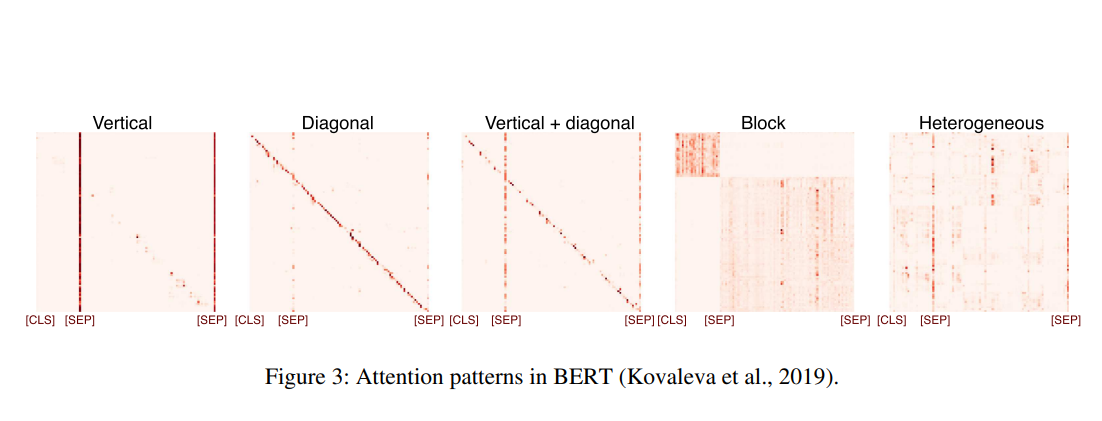
\includegraphics[width=10cm]{figure/att-pattern-bert.png}%
\end{figure}

\begin{itemize}
	\item Attempt to "understand" what the model has learned
	\item Still relevant today when seeking interpretability
\end{itemize}

\vfill

\end{frame}

% ------------------------------------------------------------------------------

\endlecture
\end{document}
